 \section{Results}\label{sec:results}
 
Our results identifies the following sources of conflicting announcements:
\begin{itemize}
\item Accidental misconfiguration
\item Malicious hijack
\item International organization
\item Content delivery network
\end{itemize}

We collected data for the first hour of every day of April 2017. This resulted in just over 700,000 BGP announcements. We found 3 hijacks and 55 misconfigurations. We identified 3 international organizations, with ASes in different countries. We found that the hijacked prefixes belonged to China, Pakistan and Bangladesh. They were falsely announced as having AS origins in Vietnam, India and India, respectively.

It is important to note that misconfigurations are potentially unconfirmed hijackings. We found some interesting patterns in the misconfigurations of specific countries. Most of the Australian misconfigurations had the AS origin 4739. The United States announced incorrect ASes for prefixes spanning several continents, including Europe, Asia and Africa. We found that most of the misconfigurations announced by Vietnam, had prefixes owned by China. The graph in Figure 3 shows the number of accidental misconfigurations by the perpetrating country.

 \begin{figure}[!htbp]
	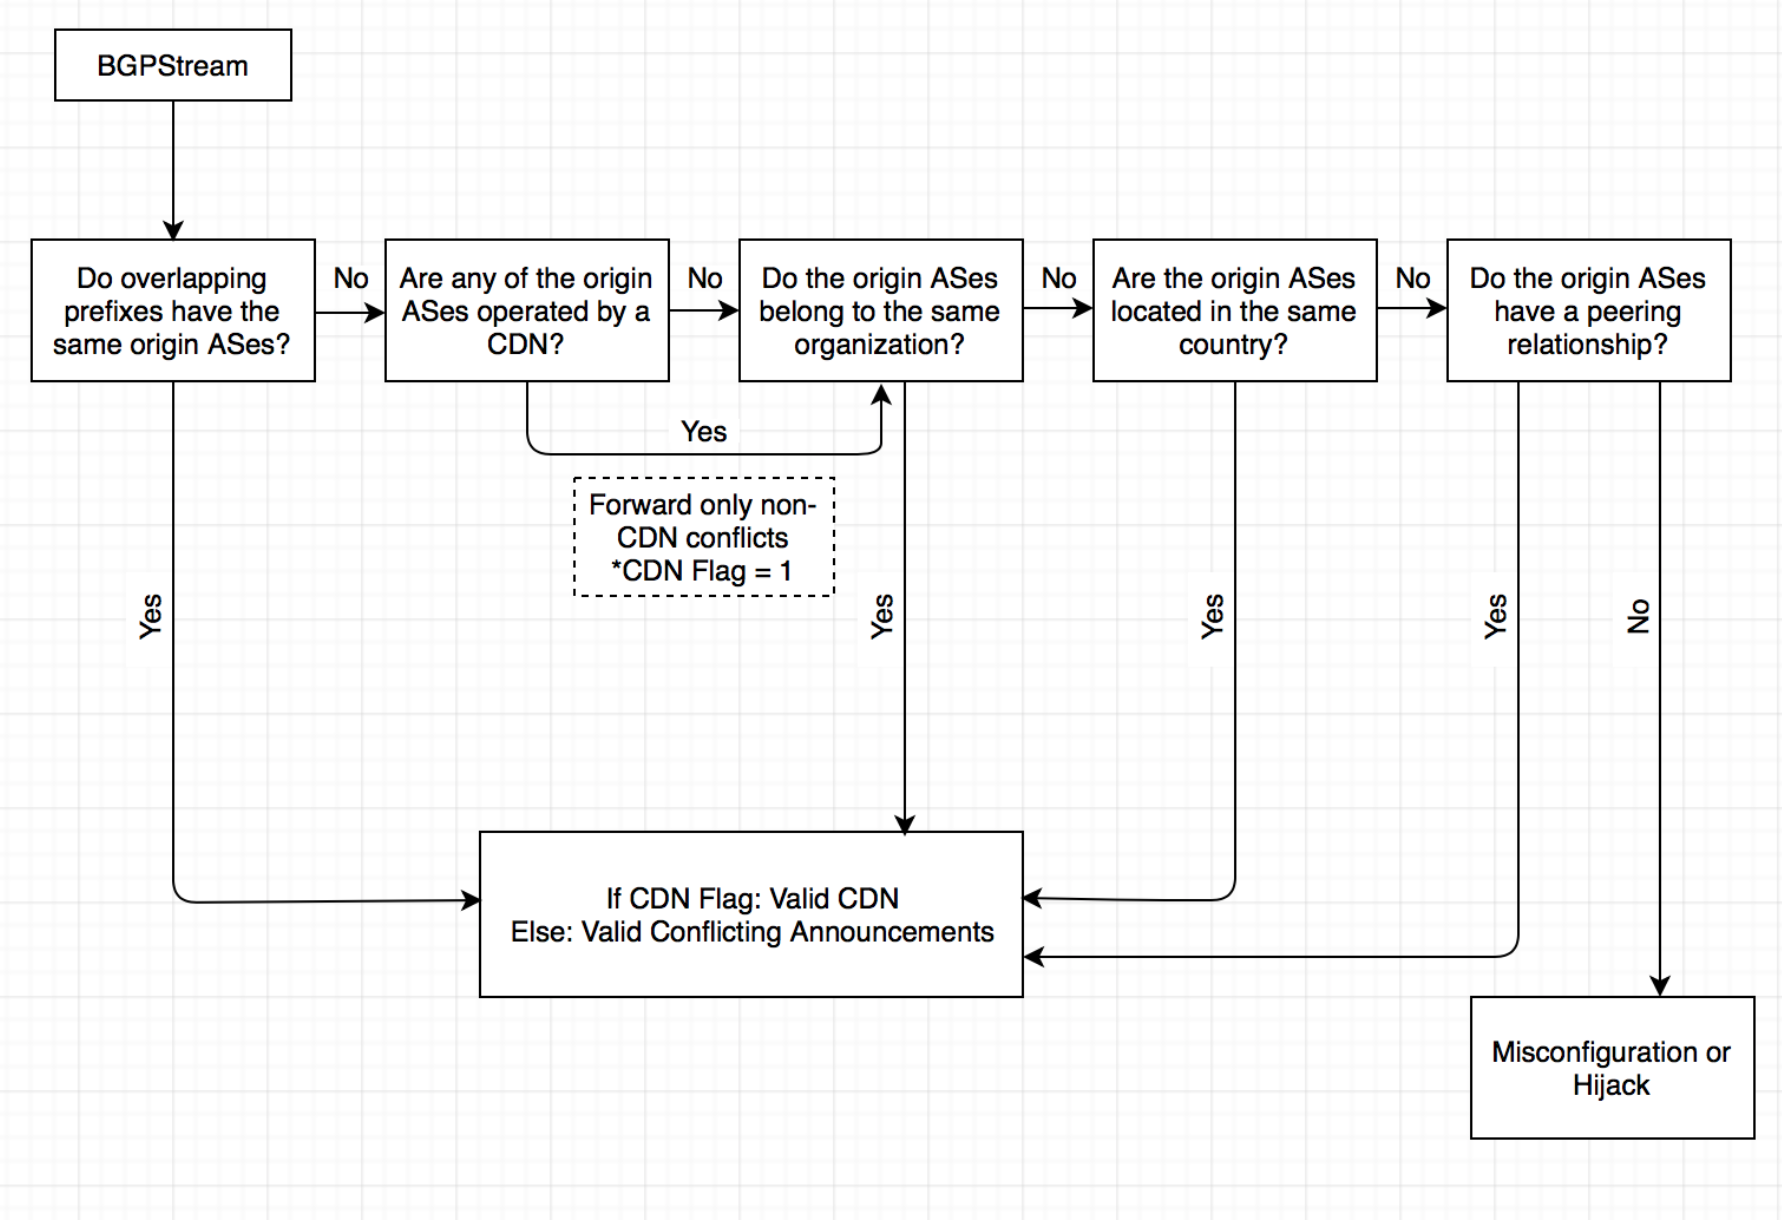
\includegraphics[width=0.5\textwidth]{flow.png}
	\caption{This figure shows the number of false announcements based on the country the announcement stemmed from.}
	\label{a:label}
\end{figure}

In addition, we see a lot of conflicting announcement for traffic engineering purposes. One AS belonging to an organization would announce more specific prefix compared to the other AS of the same organization. We ignored conflicts spanning multiple neighboring countries. For example, there were several alerts of conflicts in which AS-origins were in Colombia and Brazil, or HongKong and China. We did not label these as conflicts, and filtered them out manually.
